\documentclass[10pt,journal,twocolumn]{IEEEtran}
\usepackage{amsmath,amssymb,amsfonts}
\usepackage[T1]{fontenc}
\usepackage{graphicx}
\usepackage{booktabs}
\usepackage{multirow}
\usepackage{url}
\usepackage{textcomp}

% Number supplementary tables/figures as S1, S2, ...
\renewcommand{\thetable}{S\arabic{table}}
\renewcommand{\thefigure}{S\arabic{figure}}
\renewcommand{\thesection}{S\arabic{section}}

\begin{document}

\title{Supplementary Material for\\``Feasibility and Deployment Analysis of Tiny Machine Learning for WiFi-Based Human Activity Recognition on a Resource-Constrained Microcontroller''}
\author{Annas W. Malik and Muhammad Ahmad}
\maketitle

\noindent This document collects the secondary tables, figures, and ablations that support the main manuscript. It is referenced from the main text (for example, ``Supplementary Material, Table~S1''). All values are measured with the protocol described in the main manuscript; nothing here is required to follow the main argument, but each item is provided for completeness and reproducibility. Table and figure numbers here are prefixed with ``S''.

\section{Third-Dataset Frontier: NTU-Fi\_HAR}
To check that the accuracy-versus-cost frontier is not an artefact of UT-HAR and CSI-HAR, we ran the same pipeline on a third public dataset, NTU-Fi\_HAR~\cite{yang2023sensefi}, a clean whole-body HAR benchmark of six activities (box, circle, clean, fall, run, and walk) with three transmit-receive antennas over 114 subcarriers (stratified 80/20 split over three seeds). Table~\ref{tab:ntufi} reports the result. NTU-Fi\_HAR is saturated in the same way UT-HAR is: the tiny CNNs reach essentially perfect accuracy (100\% for the 32-channel model), the deep CNN and Transformer match them, and even the classical Random Forest reaches 99.7\%. The accuracy-versus-cost ordering therefore holds on an independent HAR corpus, and the small models remain competitive with the deep ones. As on UT-HAR, a saturated benchmark cannot expose the cross-subject gap; that is the role of the subject-independent CSI-HAR evaluation in the main text.

\begin{table}[t]
\caption{Deployability frontier on NTU-Fi\_HAR (six whole-body activities, stratified 80/20 split over three seeds). Like UT-HAR it is saturated: the tiny and classical models match the deep ones, so the accuracy-versus-cost ordering of the main frontier holds on an independent HAR corpus. The int8 sizes are larger than on the other datasets because NTU-Fi\_HAR has more input channels (342 versus 90 or 52). The classical and tiny tiers are the mean $\pm$ standard deviation over three seeds; the two deep rows are a single seed, which is why they carry no interval.}
\label{tab:ntufi}
\centering
\footnotesize
\setlength{\tabcolsep}{4pt}
\begin{tabular}{llcc}
\toprule
Model & Tier & Accuracy (\%) & int8 size (kB) \\
\midrule
Decision Tree    & classical & 95.56 $\pm$ 1.04 & emlearn C \\
Random Forest    & classical & 99.72 $\pm$ 0.20 & emlearn C \\
MLP (statistics) & classical & 98.61 $\pm$ 0.20 & emlearn C \\
Tiny CNN (8 ch)  & tiny-nn   & 99.86 $\pm$ 0.20 & 25.0 \\
Tiny CNN (16 ch) & tiny-nn   & 99.58 $\pm$ 0.59 & 46.3 \\
Tiny CNN (32 ch) & tiny-nn   & \textbf{100.00 $\pm$ 0.00} & 92.7 \\
Deep CNN         & deep      & 100.00 & 213.4 \\
Transformer      & deep      & 99.58 & 166.8 \\
\bottomrule
\end{tabular}
\end{table}

\section{Classical Output Parity: scikit-learn versus emlearn C}
The faithfulness check that the main text applies to the neural int8 models applies equally to the classical tier, which is deployed as emlearn C rather than TensorFlow Lite. We compared the emlearn C export against the trained scikit-learn model over the full real test set of each dataset (Table~\ref{tab:emlearnparity}): using the floating-point export the Decision Tree and statistics MLP are bit-exact on both datasets, and the Random Forest matches on 100\% of CSI-HAR and 98.6\% of UT-HAR test windows, the small residual coming from scikit-learn averaging per-tree probabilities where the C export resolves ties by tree vote. The classical models therefore reproduce their reference predictions on-device.

\begin{table}[t]
\caption{Output parity between the scikit-learn classical models and their emlearn C export, as the exact-match rate over the full real test set (floating-point export). Decision Tree and statistics MLP are bit-exact; the Random Forest differs only on 1.4\% of UT-HAR windows.}
\label{tab:emlearnparity}
\centering
\footnotesize
\begin{tabular}{llcc}
\toprule
Dataset & Model & Exact match (\%) & Test windows \\
\midrule
CSI-HAR & Decision Tree    & 100.0 & 420 \\
CSI-HAR & Random Forest    & 100.0 & 420 \\
CSI-HAR & MLP (statistics) & 100.0 & 420 \\
UT-HAR  & Decision Tree    & 100.0 & 500 \\
UT-HAR  & Random Forest    & 98.6  & 500 \\
UT-HAR  & MLP (statistics) & 100.0 & 500 \\
\bottomrule
\end{tabular}
\end{table}

\section{Operators Behind the Deployment Failures}
Table~\ref{tab:unsupported} lists the specific operators responsible for the deep-tier deployment failures discussed in the main text. The recurrent and state-space models fail at int8 conversion because their fused or dynamic-tensor operators are outside the TFLM builtin set and would require the Select-TF-ops (flex) path, which the ESP32 runtime does not provide. The Chebyshev-KAN converts but its \texttt{FILL} node fails to prepare at \texttt{AllocateTensors}. The convolutional and attention feed-forward models use only builtin operators and deploy.

\begin{table}[t]
\caption{Operators responsible for the deployment failures, by model and failing stage.}
\label{tab:unsupported}
\centering
\footnotesize
\setlength{\tabcolsep}{4pt}
\begin{tabular}{lll}
\toprule
Model & Failing stage & Blocking operator(s) \\
\midrule
BiGRU           & int8 conversion   & \texttt{CudnnRNNV3} (fused GRU) \\
Lightweight-SSM & int8 conversion   & \texttt{TensorListReserve}, \texttt{While} \\
Chebyshev-KAN   & \texttt{AllocateTensors} & \texttt{FILL} (prepare fails) \\
\midrule
CNN, Transformer & none (deploy)   & builtin operators only \\
\bottomrule
\end{tabular}
\end{table}

\section{CPU-Frequency Scaling}
The classic ESP32 boots at 160\,MHz under the default ESP-IDF configuration but can run at 240\,MHz, and the choice matters for a latency budget. Table~\ref{tab:cpufreq} compares the two operating points for representative models: at 240\,MHz every model is about a third faster, with the compute-bound tiny CNNs scaling close to the 1.5$\times$ clock ratio and the deep CNN scaling less (1.26$\times$) because a larger share of its time is spent moving activations rather than computing. All on-device results in the main text use 240\,MHz. We do not claim a simple energy relationship between the two clocks: the active current itself changes with frequency, so the net per-inference energy at 160\,MHz (lower power but longer latency) is an empirical question we do not settle here.

\begin{table}[t]
\caption{CPU-frequency scaling on the classic ESP32: per-inference latency at 160\,MHz (the ESP-IDF default) and at 240\,MHz (full speed, used for all main-text results).}
\label{tab:cpufreq}
\centering
\footnotesize
\setlength{\tabcolsep}{4pt}
\begin{tabular}{llccc}
\toprule
Model & Dataset & 160\,MHz (ms) & 240\,MHz (ms) & Speedup \\
\midrule
Tiny CNN (8 ch)  & UT-HAR  & 21.4  & 14.1  & 1.52$\times$ \\
Tiny CNN (16 ch) & CSI-HAR & 30.2  & 20.2  & 1.50$\times$ \\
Deep CNN         & CSI-HAR & 306.8 & 243.5 & 1.26$\times$ \\
Deep Transformer & CSI-HAR & 476.1 & 320.7 & 1.48$\times$ \\
\bottomrule
\end{tabular}
\end{table}

\section{Compiler Optimization and the Optimized Kernel Library}
Two build-time factors were isolated. The compiler optimization level barely matters for this workload: rebuilding the 16-channel tiny CNN and the deep CNN with size optimization ($-$Os) instead of the default performance optimization ($-$O2) changed latency by less than 3\% (if anything $-$Os was marginally faster, 28.1 against 29.7\,ms for the tiny CNN and 221 against 226\,ms for the deep CNN on UT-HAR), left the tensor arena unchanged, and reduced the firmware image by about 1.5\%. Almost all of the time is spent inside the quantized TFLM kernels, which the compiler optimizes similarly at either level. The one factor that dominates on-device speed is the optimized kernel library: the \texttt{esp-tflite-micro} runtime enables ESP-NN, Espressif's Xtensa-optimized int8 kernels, by default, and all main-text measurements use it. Rebuilding with ESP-NN disabled (portable reference kernels) slowed the 16-channel tiny CNN on CSI-HAR from 20.2\,ms to 275.7\,ms, a 13.6$\times$ penalty, and made the deep CNN so slow (over 5\,s per inference) that a single inference trips the task watchdog. The optimized kernels are therefore essential rather than optional for real-time CSI inference on this chip, and their effect dwarfs both the clock (1.5$\times$) and the compiler flag. CMSIS-NN, the comparable library, targets ARM Cortex-M cores and does not apply to the Xtensa LX6; ESP-NN is its Xtensa counterpart.

\section{Tensor-Arena Ablations}
Table~\ref{tab:arena} sweeps the arena given to the 16-channel tiny CNN on CSI-HAR, whose true requirement is 8488 bytes. The behaviour is a sharp threshold: below 8488 bytes the interpreter cannot allocate and the model does not deploy, while at or above it the model fits, reports the same 8488-byte peak, and runs at the same latency (20.24\,ms) regardless of how much extra arena is provided. Over-provisioning the arena only wastes RAM. The ablation also surfaced a byte-addressability constraint that a bare-device study exposes and a PSRAM-equipped one would not: the arena must be forced into byte-addressable internal RAM with \texttt{MALLOC\_CAP\_8BIT}, because a small arena requested only as generic internal memory can be placed in instruction RAM (32-bit access only), where int8 tensor access faults.

\begin{table}[t]
\caption{Tensor-arena-size ablation for the 16-channel tiny CNN on CSI-HAR (true requirement 8488 bytes, at 240\,MHz).}
\label{tab:arena}
\centering
\footnotesize
\setlength{\tabcolsep}{6pt}
\begin{tabular}{ccc}
\toprule
Requested arena (B) & Fits & Latency (ms) \\
\midrule
7168  & no  & n/a \\
8192  & no  & n/a \\
8448  & no  & n/a \\
8704  & yes & 20.24 \\
16384 & yes & 20.24 \\
32768 & yes & 20.25 \\
\bottomrule
\end{tabular}
\end{table}

To see where the arena goes within the two deep models, we instrumented the interpreter with the recording allocator and read back the arena composition (Table~\ref{tab:arenabreakdown}). The allocator splits the arena into a \emph{head} (the working buffer for intermediate activations) and a \emph{tail} of persistent structures (per-operator node records, quantization metadata, and kernel scratch). The deep CNN has 16 operators, a small 4.2\,kB tail, and a head that scales gently with the input. The Transformer has 55 operators, a much larger tail (14 to 18\,kB), and a head that scales with the square of the sequence length, reaching 36.9\,kB on the 64-step CSI-HAR window. This is why the Transformer needs the most arena of any model we deploy and confirms, from the memory side, the latency story of the main text.

\begin{table}[t]
\caption{Tensor-arena composition of the two deployable deep models, from the recording allocator (kB). \emph{Head} is the activation working buffer; \emph{tail} is the persistent structures; \emph{Ops} is the operator count.}
\label{tab:arenabreakdown}
\centering
\footnotesize
\setlength{\tabcolsep}{5pt}
\begin{tabular}{llcccc}
\toprule
Model & Dataset & Total (kB) & Head (kB) & Tail (kB) & Ops \\
\midrule
Deep CNN    & UT-HAR  & 10.1 & 6.0  & 4.1  & 16 \\
Deep CNN    & CSI-HAR & 12.1 & 8.0  & 4.1  & 16 \\
Transformer & UT-HAR  & 24.1 & 10.0 & 14.0 & 55 \\
Transformer & CSI-HAR & 54.1 & 36.0 & 18.0 & 55 \\
\bottomrule
\end{tabular}
\end{table}

\section{Memory with the Radio Active}
Table~\ref{tab:wifimem} reports on-device memory and latency with the radio off versus WiFi active (station mode). The tensor arena is unchanged by the radio; WiFi initialization drops the largest free internal block from 152\,kB to 108\,kB, and during the live run it is about 88 to 92\,kB. The heap left after the arena is the practical headroom for application code and network buffers, which is tight for the deep Transformer. Latency stays within a millisecond of the radio-off value because inference is CPU-bound and the idle driver does not contend for compute.

\begin{table}[t]
\caption{On-device memory and latency with the radio off versus WiFi active (station mode), classic ESP32 at 240\,MHz.}
\label{tab:wifimem}
\centering
\footnotesize
\setlength{\tabcolsep}{3.5pt}
\begin{tabular}{lccccc}
\toprule
Model & Arena (kB) & Lat.\ off (ms) & Lat.\ WiFi (ms) & Heap @108\,kB & Heap @$\sim$90\,kB \\
\midrule
Tiny CNN (16 ch) & 8.3 & 20.2  & 20.1  & $\sim$100\,kB & $\sim$82\,kB \\
Deep CNN         & 12  & 243.5 & 244.6 & $\sim$96\,kB  & $\sim$78\,kB \\
Deep Transformer & 54  & 320.7 & 322.0 & $\sim$54\,kB  & $\sim$36\,kB \\
\bottomrule
\end{tabular}
\end{table}

\section{Supplementary Figures}
Figures~\ref{fig:accuracy}, \ref{fig:complexity}, and \ref{fig:memory} present the classical and tiny tiers graphically: accuracy across datasets, model complexity on a logarithmic axis, and the measured peak tensor arena of every deployable model against the roughly 150\,kB contiguous block the runtime exposes. The numerical values behind these plots are in the main-text tables.

\begin{figure}[tbp]
\centering
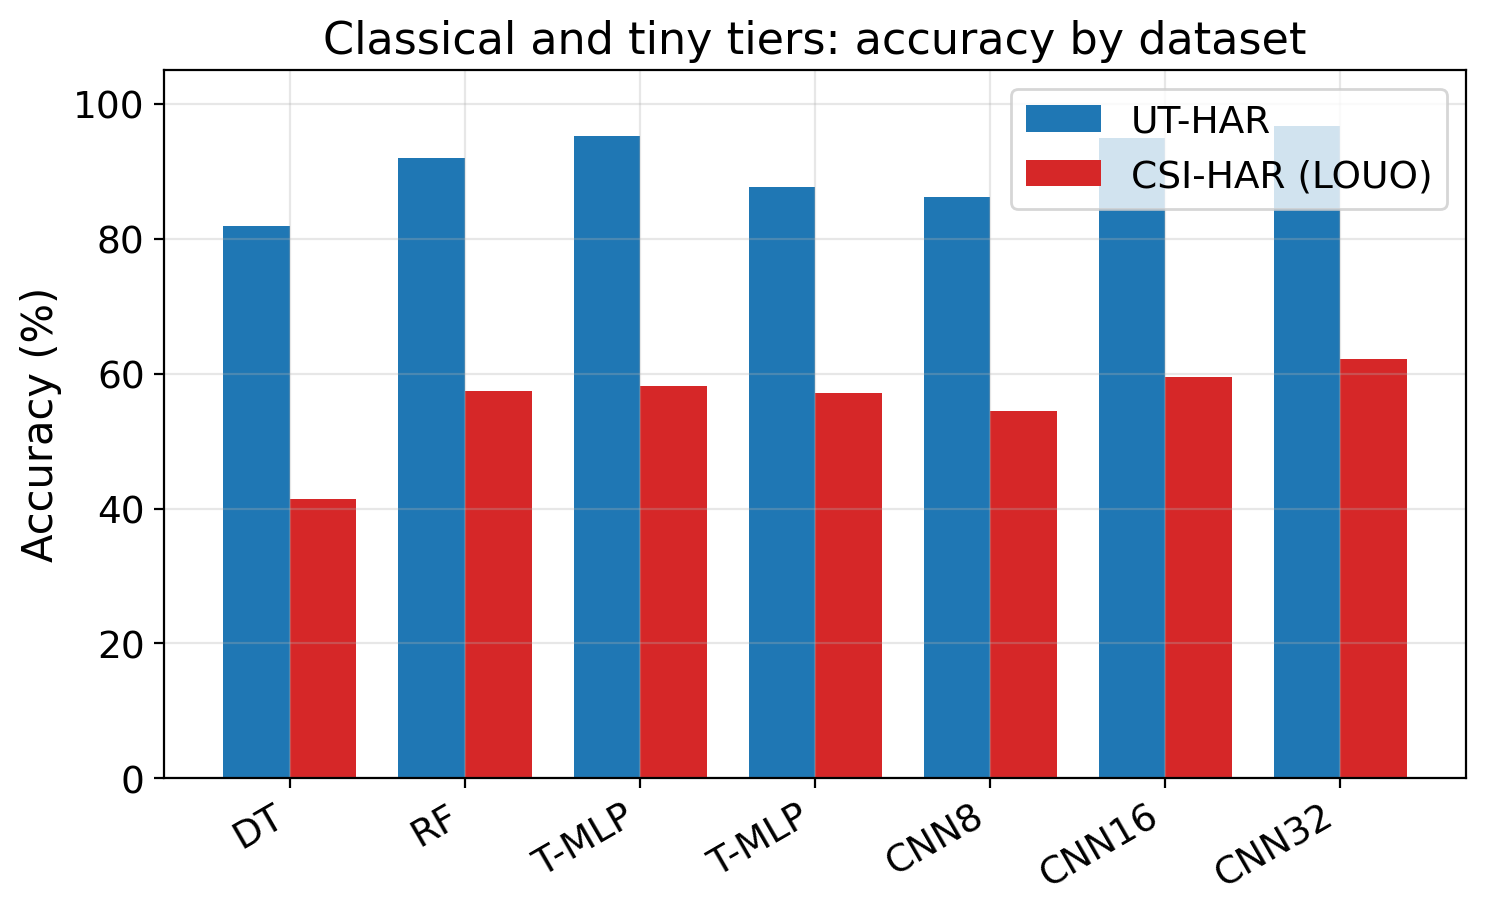
\includegraphics[width=\columnwidth]{fig_accuracy.png}
\caption{Accuracy of the classical and tiny tiers across UT-HAR and CSI-HAR. Accuracy is consistently lower on CSI-HAR, which has fewer samples per class and is evaluated under a subject-independent split.}
\label{fig:accuracy}
\end{figure}

\begin{figure}[tbp]
\centering
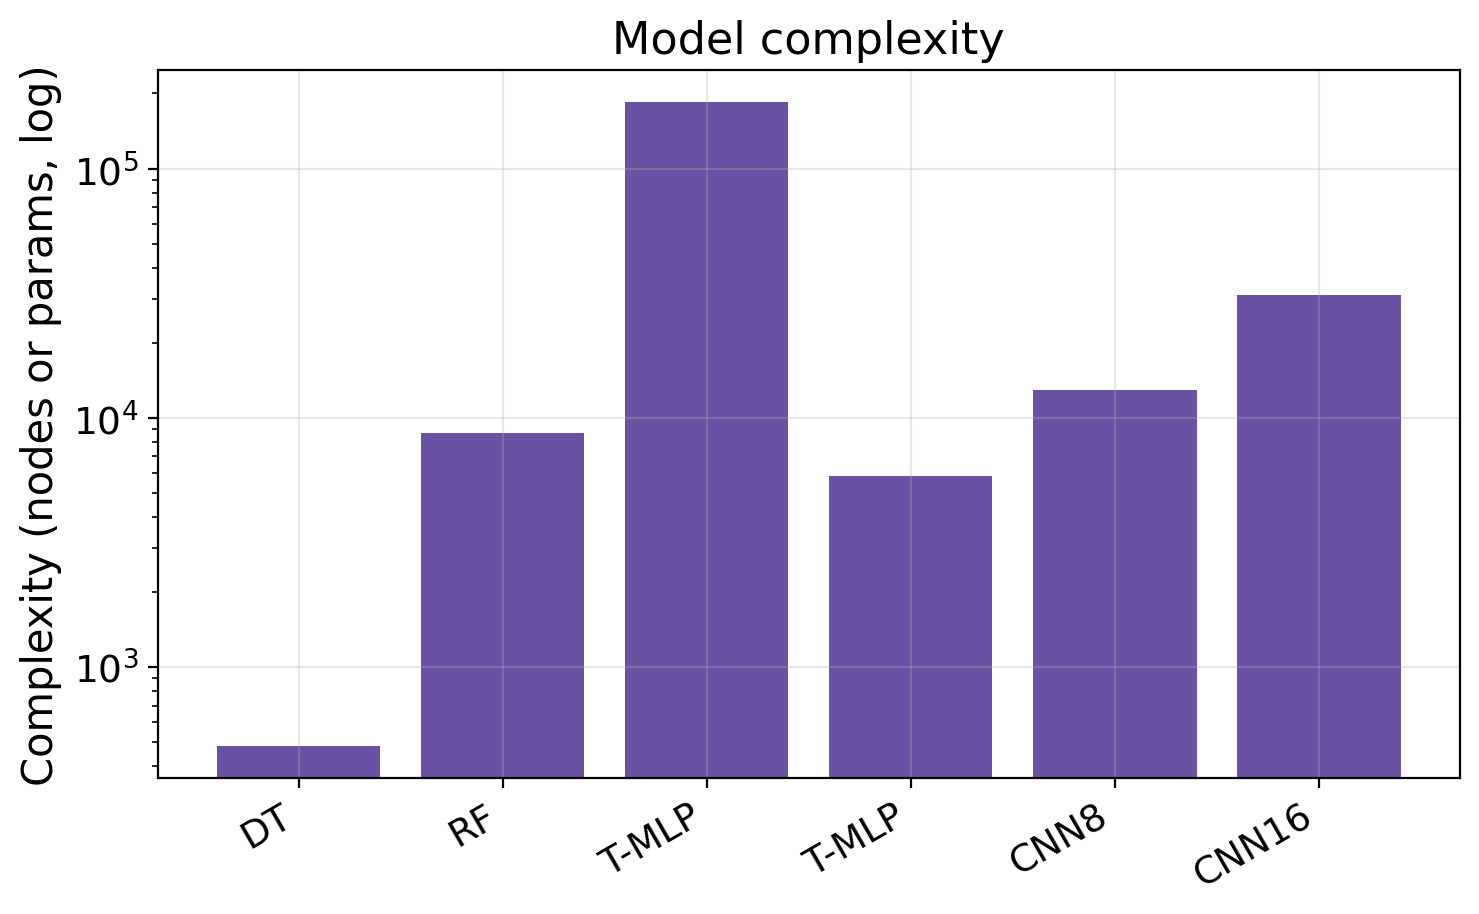
\includegraphics[width=\columnwidth]{fig_complexity.png}
\caption{Model complexity on a logarithmic axis (tree node count or network parameter count). The classical learners are one to three orders of magnitude smaller than the networks.}
\label{fig:complexity}
\end{figure}

\begin{figure}[tbp]
\centering
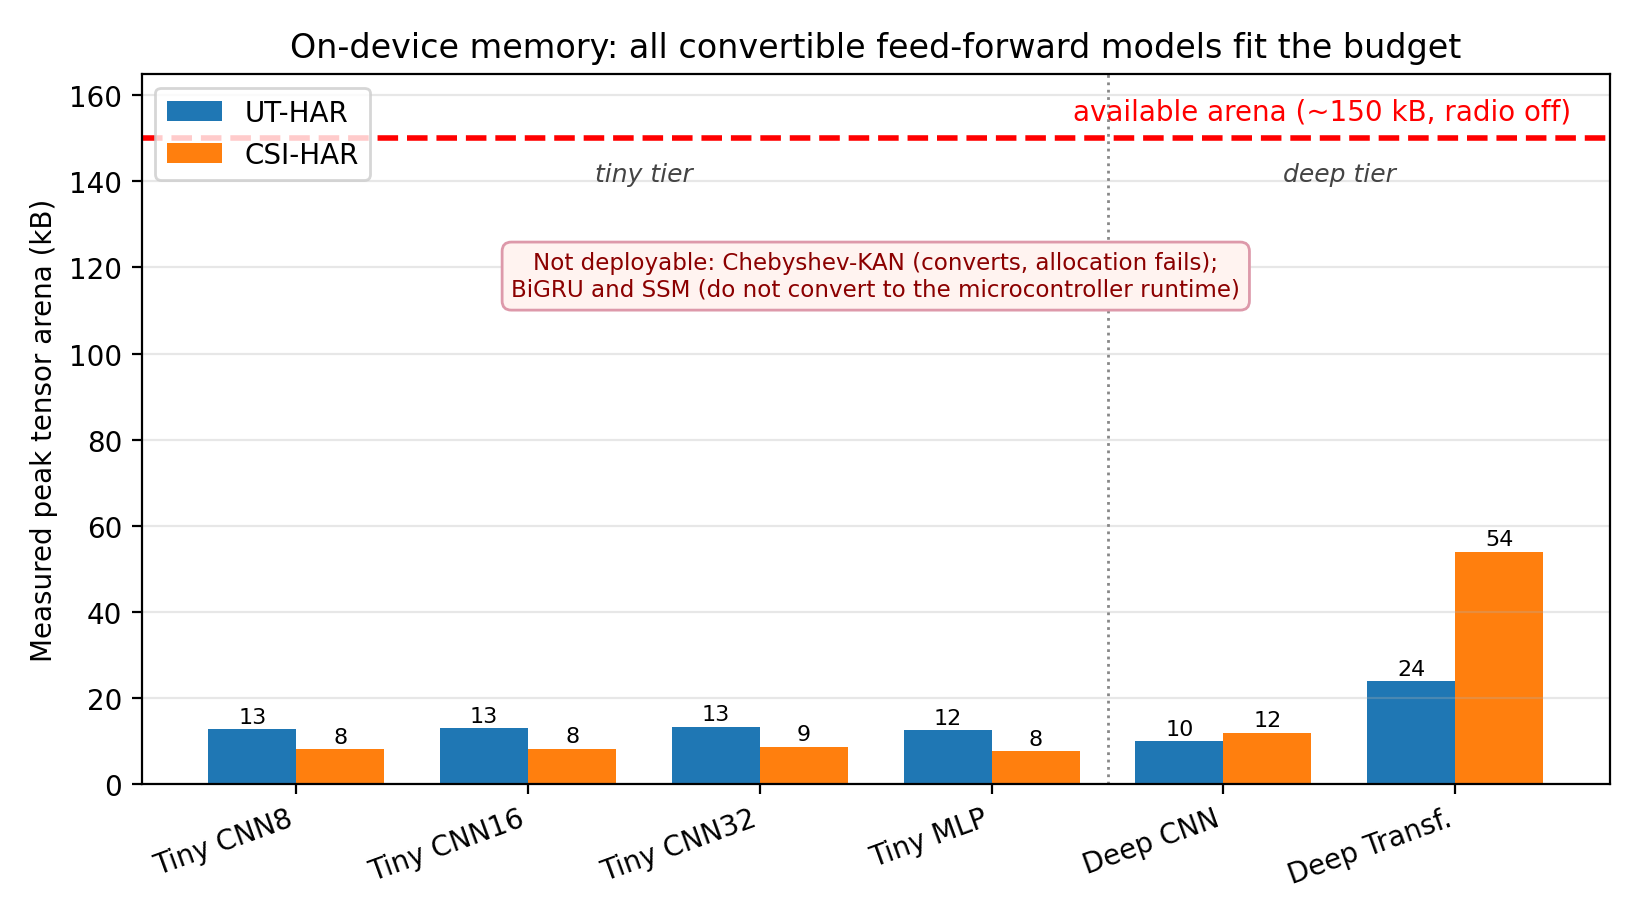
\includegraphics[width=\columnwidth]{fig_memory.png}
\caption{Measured peak tensor arena of the deployable models on the classic ESP32, against the roughly 150\,kB contiguous block the runtime exposes (dashed line). Every convertible feed-forward model fits with a large margin, including the deep CNN (10 to 12\,kB) and Transformer (24 to 54\,kB). The Chebyshev-KAN converts but fails to allocate, and the recurrent and state-space models do not convert; neither is shown.}
\label{fig:memory}
\end{figure}

\begin{thebibliography}{1}
\bibitem{yang2023sensefi}
J. Yang, X. Chen, H. Zou, D. Wang, Q. Xu, and L. Xie, ``SenseFi: a library and benchmark on deep-learning-empowered WiFi human sensing,'' \emph{Patterns}, vol. 4, no. 3, p. 100703, Mar. 2023.
\end{thebibliography}

\end{document}
